\subsection{Results} \label{results}
The participants had varied experience with Autodesk Maya, ranging from six months to six years. In Unity, their experience ranged from none at all to more than a year.

%Four of the six participants reported having between one and three years of experience with Autodesk Maya. One participant had between four and six years of experience, and another had seven or more years of experience. Only one participant had more than one year of experience with Unity; another had between six and twelve months of experience with it. The rest reported to have less than six months of experience with Unity.

%When asked if they \textit{"felt empowered using the tool"}, two participants responded \textit{strongly agreed} and four participants responded \textit{agreed}.

The coded data gathered from video analysis shows that the number of events tagged with \textit{confusion} and \textit{problem} in the task and creative phase, which can be seen in Figure \ref{fig:codedgraph}. In the task phase, 23 events were tagged as \textit{confusion} and 15 as \textit{problem}. In the creative phase, 7 events were tagged as \textit{confusion} and 4 as \textit{problem}. This is an increase of 53.4\% and 57.8\% for \textit{confusion} and \textit{problem}, respectively.

\begin{figure}[htbp]
\centering
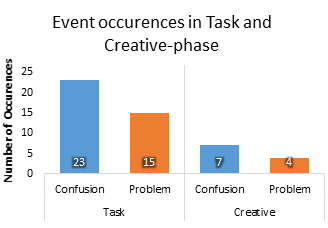
\includegraphics[width=0.45\textwidth]{Pics/codedgraph2}
\caption{Number of occurrences for confusion and problem in both the task and creative-phase.}
\label{fig:codedgraph}
\end{figure}

When asked if the participants \textit{"felt empowered using the tool"}, four participants \textit{agreed}, while the remaining two \textit{strongly agreed}. When asked if they \textit{"felt restricted using the tool"}, five participants \textit{disagreed} while the remaining participant \textit{strongly disagreed}.

To find out how efficient the participants felt using the FCT, we asked them if they felt they \textit{"got the tasks done quickly"}. Four participants \textit{agreed} and two \textit{strongly agreed}. To find out how effective the participants felt using our tool, we asked them if they \textit{"felt the tool allowed them to complete the tasks well"}. Three participants \textit{agreed} and three \textit{strongly agreed}.

When asked about the preview features, five participants found them \textit{very useful}, and one found it \textit{somewhat useful}. The participants were also asked whether they preferred the \textit{be the camera} or the \textit{snapshot} feature. Four named\textit{ be the camera} and two named \textit{snapshot}. Furthermore, three participants noted the \textit{be the camera} feature as their overall favourite feature, while the \textit{slider preview} was the favourite for the other three participants. 